\documentclass{beamer}

\usetheme{Goettingen}

\usepackage[french]{babel}
\usepackage[utf8]{inputenc}
\usepackage[T1]{fontenc}
\usepackage{lmodern}
\usepackage{graphicx}
\usepackage{color}
\usepackage{amsmath, amssymb}
\newcommand{\R}{\mathbb{R}}
\newcommand{\Z}{\mathbb{Z}}

\author{Gaspard Jankowiak \quad Antoine Levitt\\ Tuteur : Antoine Girard}
\title{{\textbf{\textcolor{black}{Projet Spécialité Ensimag 2A}}}\vspace{1cm}\\ {Ajustement d'opinions et création de communautés dans des réseaux
sociaux}}
\date{19 juin 2009}

\begin{document}
\begin{frame}
	\maketitle
\end{frame}

\begin{frame}{Graphes utilisés}{Graphes réels}
	\begin{center}
		\begin{tabular}[h]{cc}
			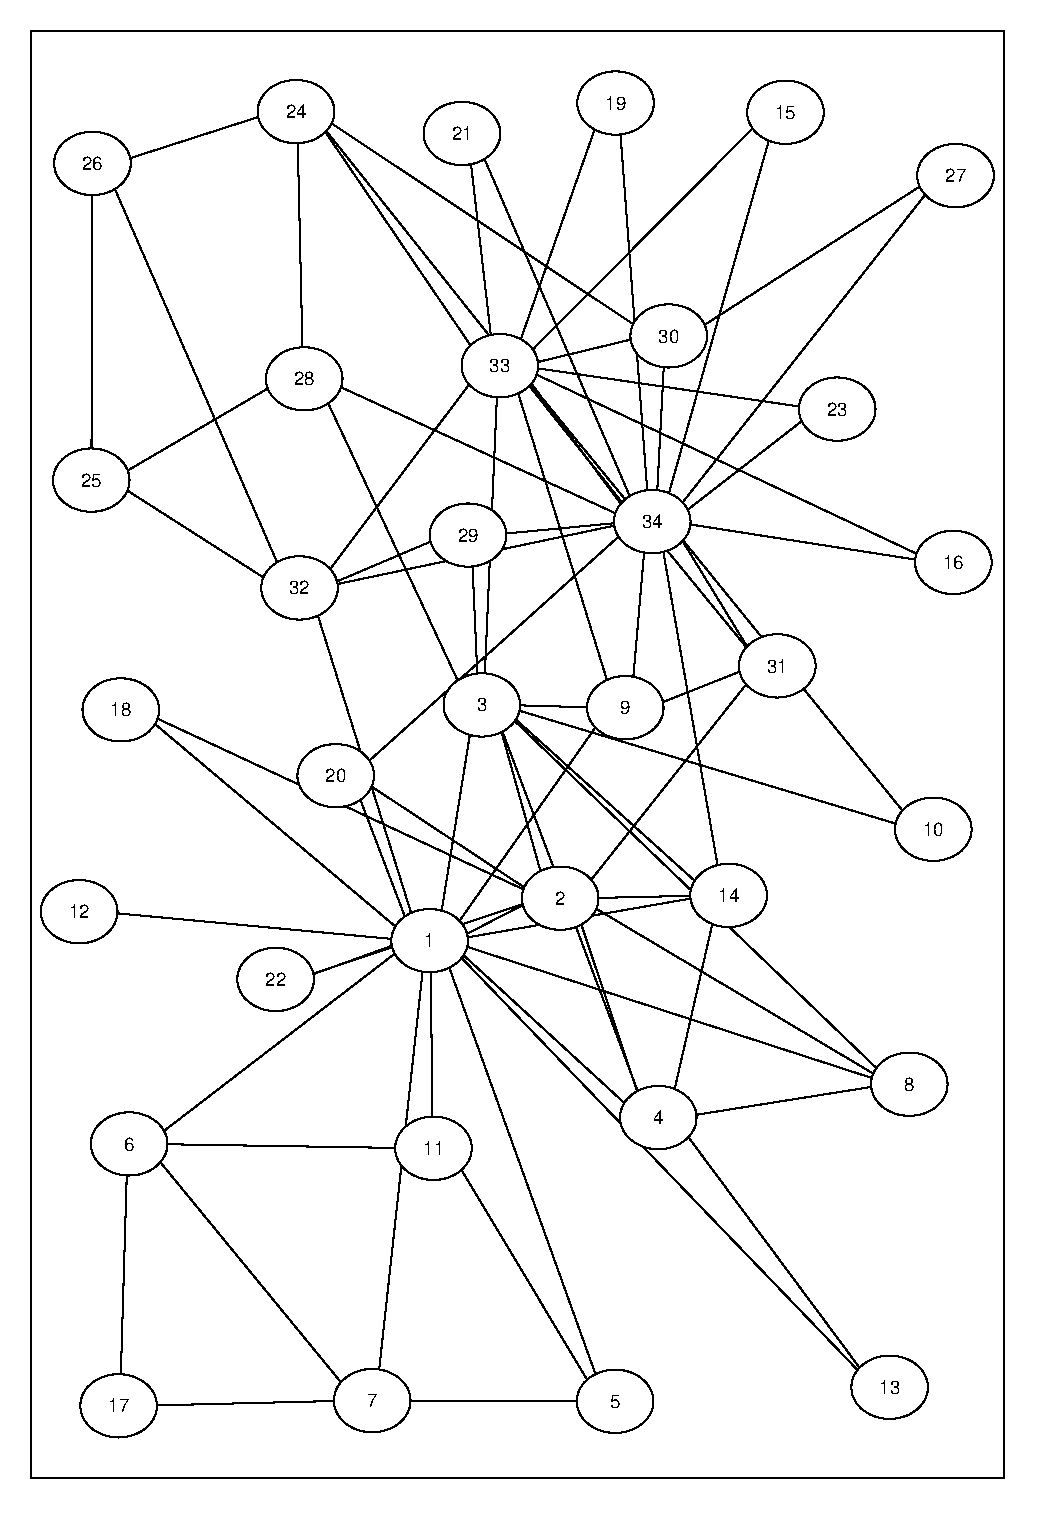
\includegraphics[width=0.4\textwidth]{pres-za}&
			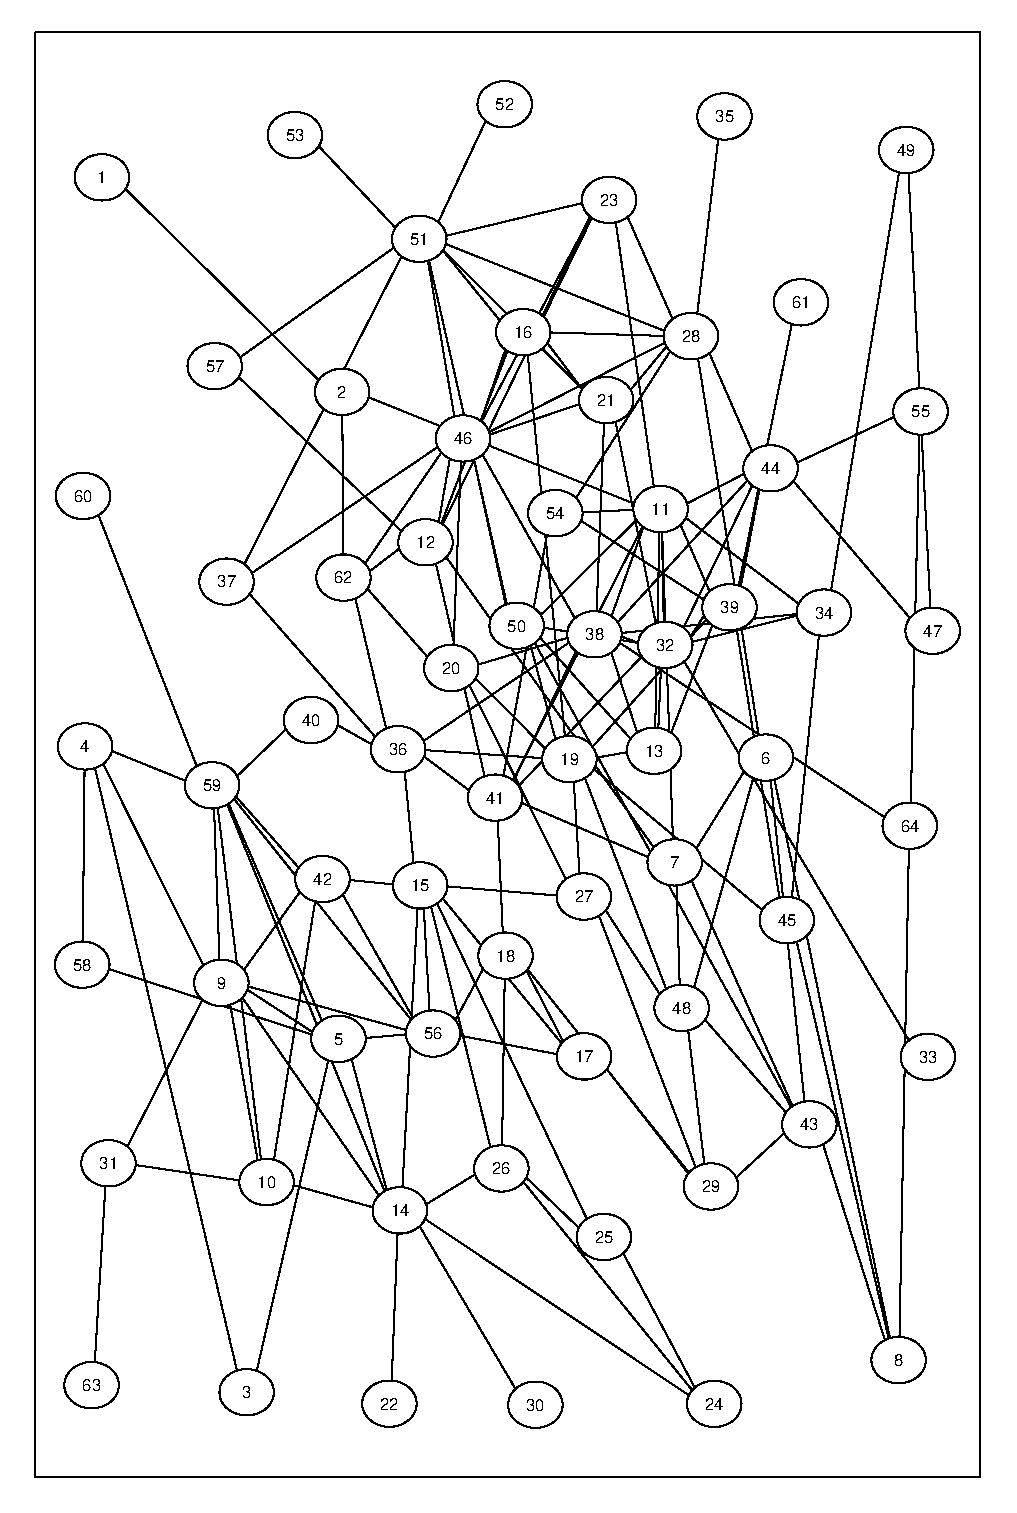
\includegraphics[width=0.4\textwidth]{pres-do}
			\\
			Club de karaté Zachary & Banc de dauphins
		\end{tabular}
	\end{center}
\end{frame}

\begin{frame}{Evolution temporelle}{Consensus : $\rho > \lambda_2$} 
	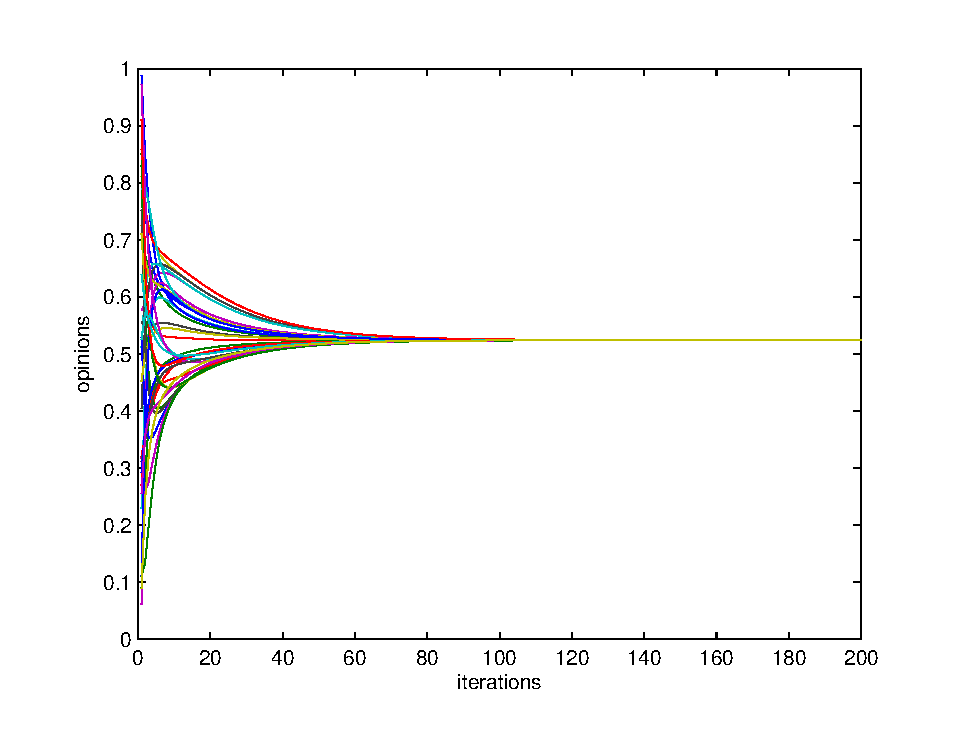
\includegraphics[width=\textwidth]{evolution_ok}
\end{frame}
\begin{frame}{Evolution temporelle}{Apparition de groupes : $\rho < \lambda_2$}
	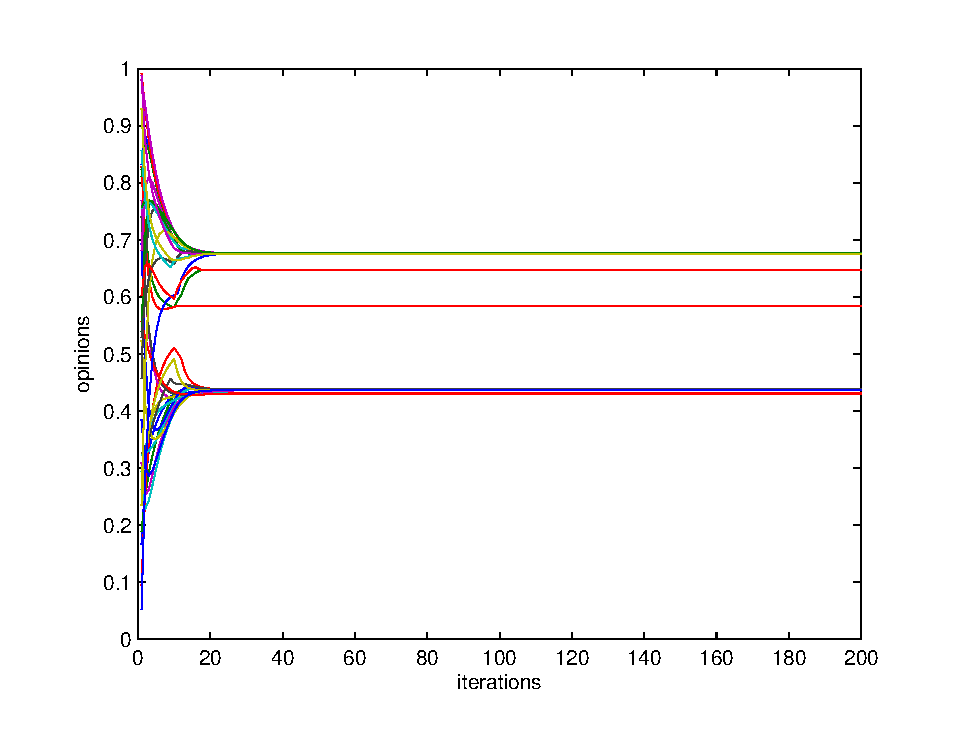
\includegraphics[width=\textwidth]{evolution_clusters}
\end{frame}

\begin{frame}{Détection des groupes}
	Groupes $\equiv$ composantes connexes du graphe :
	$$N'(t)=\bigcup_i N'_i(t).$$

	Rappel : $N'_i(t) = \{j \in N_i, ||x_i - x_j|| < R \rho^t\}.$
\end{frame}

\begin{frame}{Formation de groupes}
	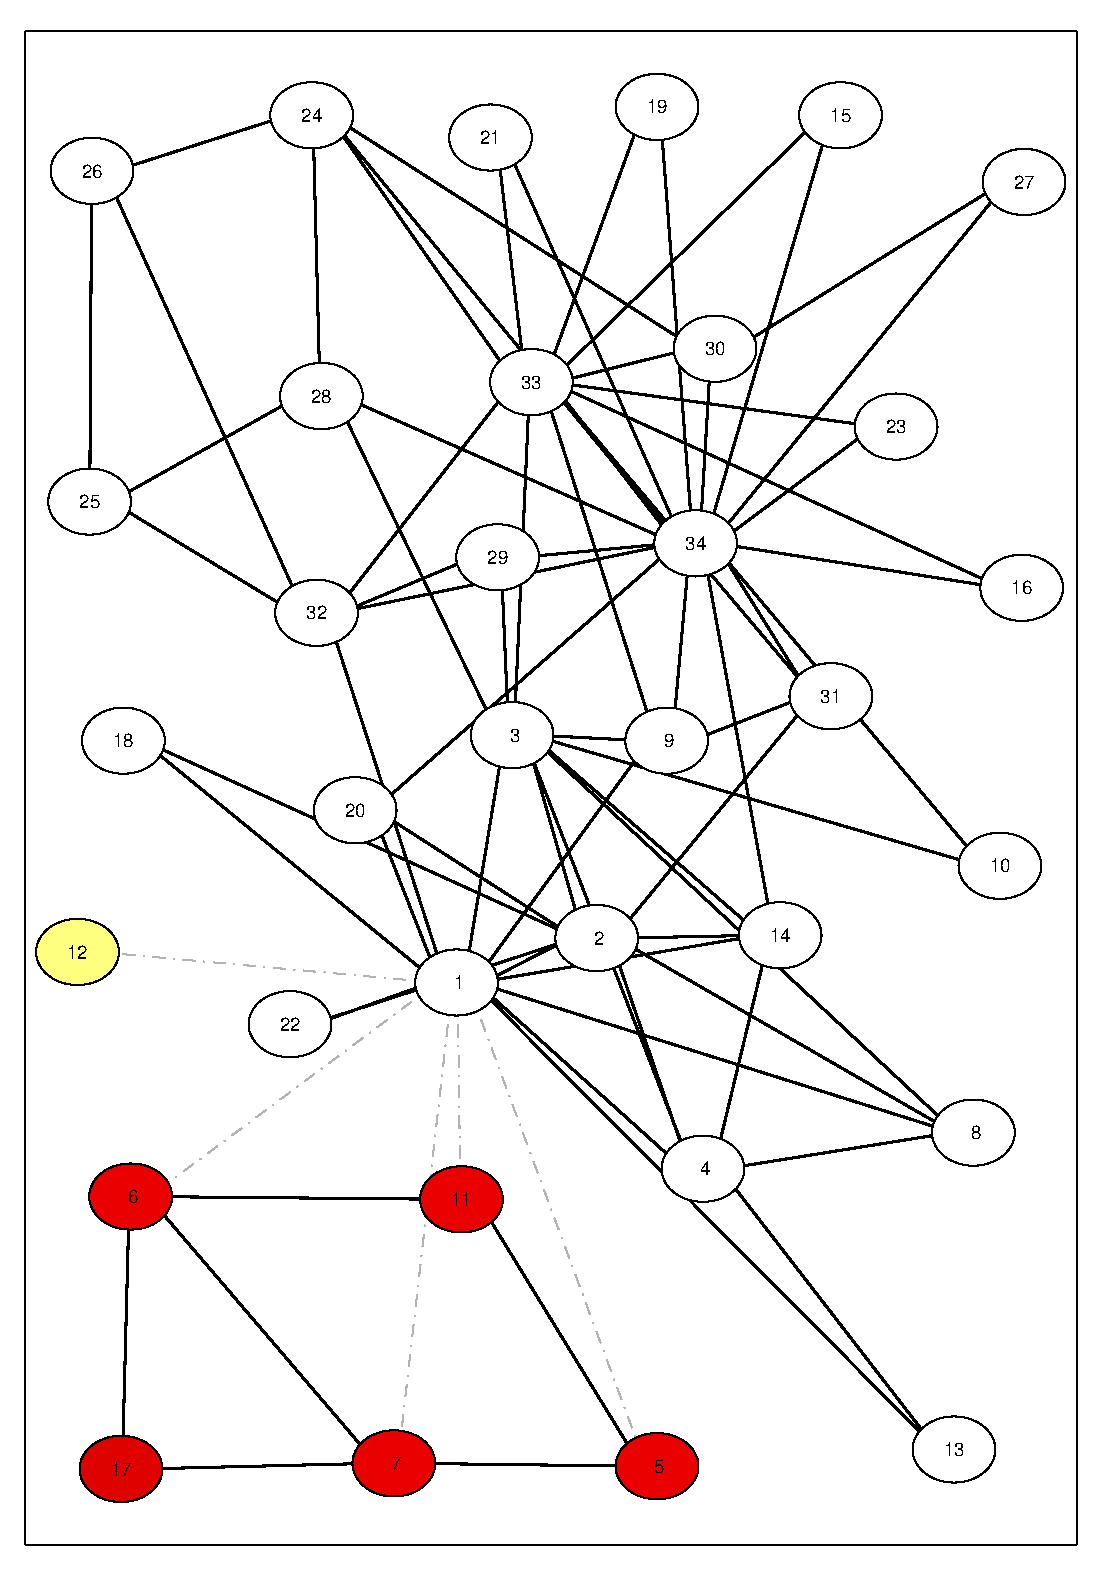
\includegraphics[width=.5\textwidth]{za-m1-3}
	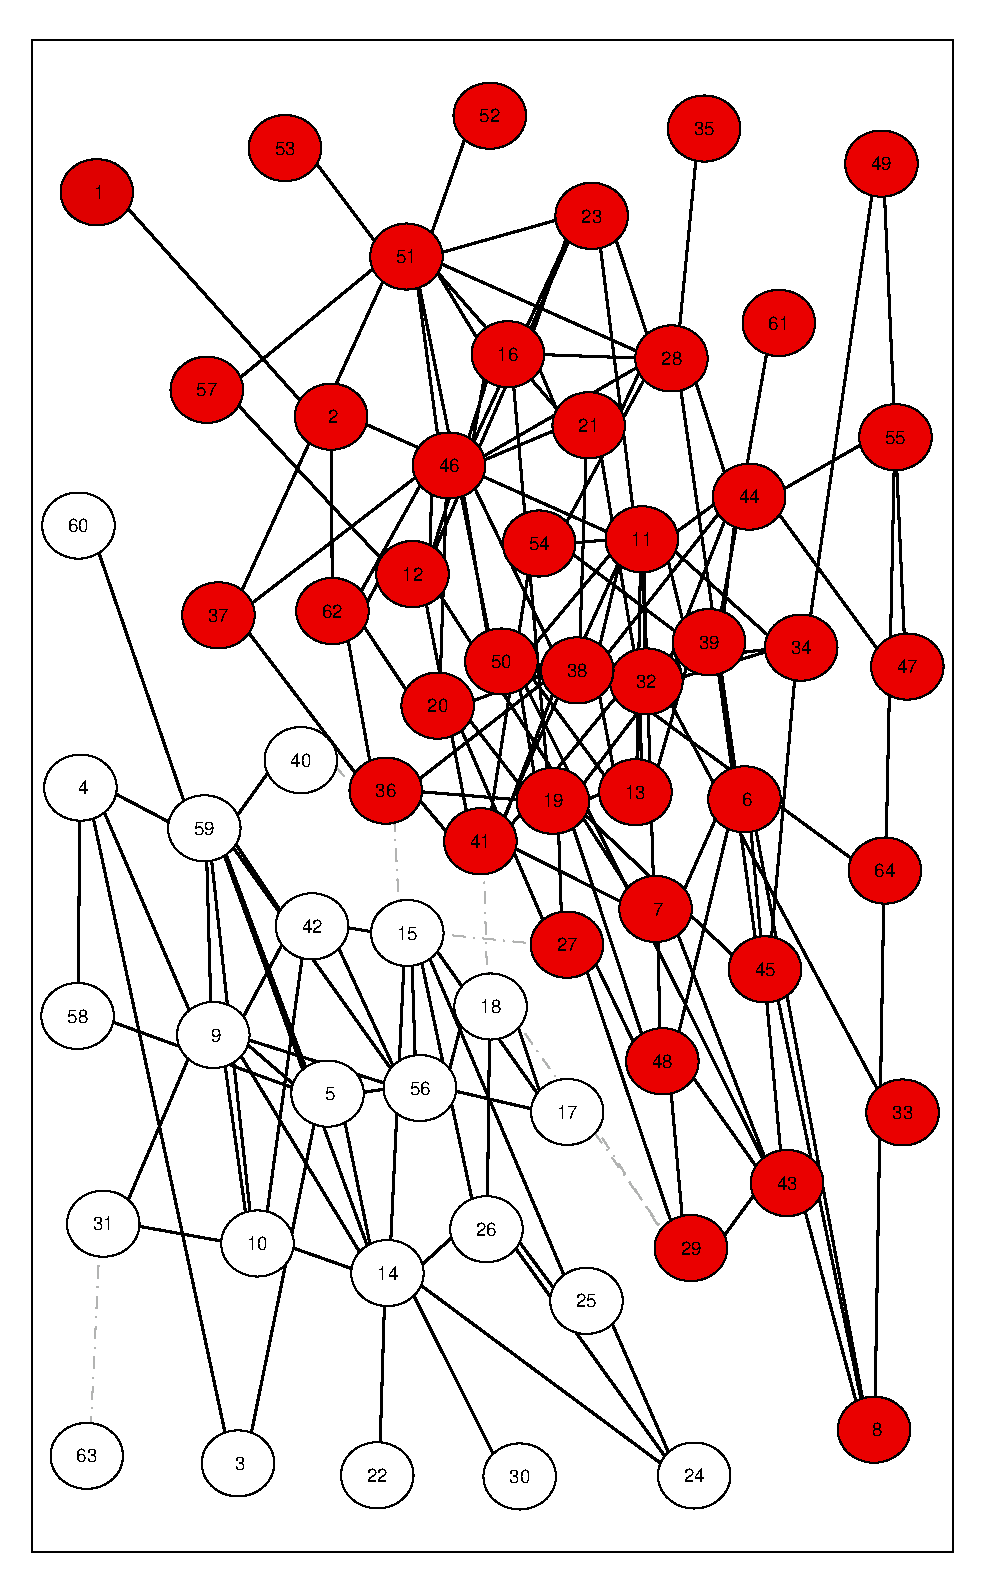
\includegraphics[width=.5\textwidth]{do-m1-3}
\end{frame}

\begin{frame}{Bifurcation pour $\rho = \lambda_2$}{Graphe club de karaté de Zachary, $\rho = 0,953$}
	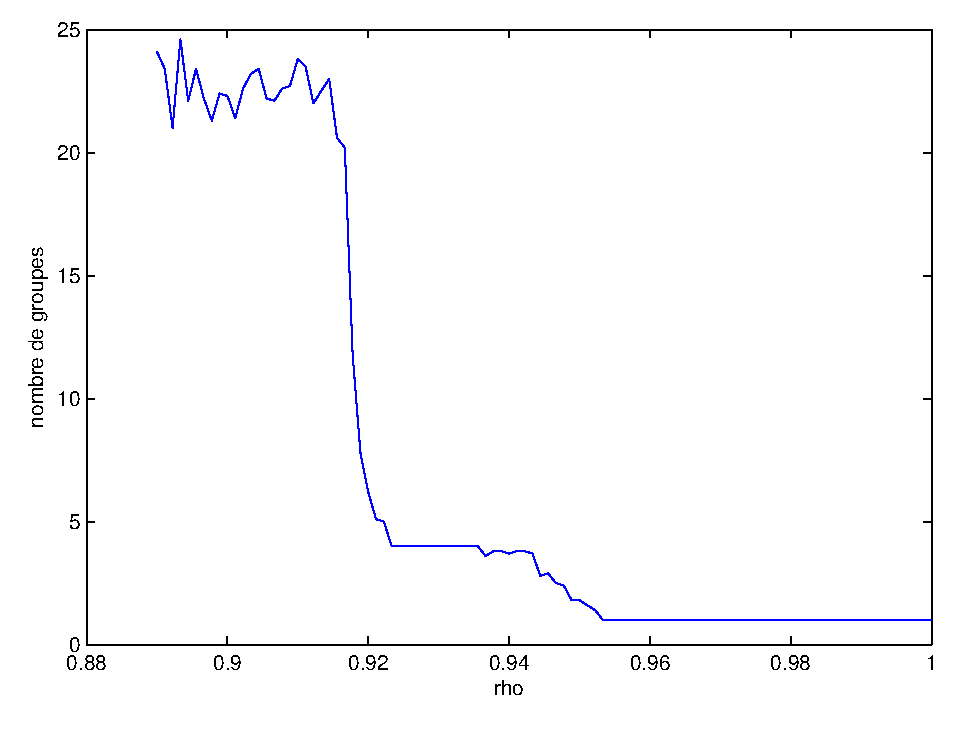
\includegraphics[width=\textwidth]{bifur}
\end{frame}


\end{document}
